% ------------------------------------------------------------
% File: figures/fig-iteration-2-mask-comparison.tex
% Iteration 1 to Iteration 2 mask geometry comparison
% ------------------------------------------------------------

\begin{figure}[htbp]
  \centering
  \begin{tikzpicture}[
    font=\footnotesize,
    imglabel/.style={draw, fill=white, line width=0.35pt, inner xsep=4pt,
      inner ysep=2pt, font=\small\bfseries},
    change/.style={-Latex, line width=1.2pt},
    highlight/.style={dashed, draw=red!80!black, line width=1.6pt},
    boxarrow/.style={-Latex, draw=red!80!black, line width=1.5pt},
    connectorlabel/.style={draw, fill=white, line width=0.35pt, inner xsep=4pt,
      inner ysep=2pt, font=\footnotesize\bfseries, text=red!80!black,
      align=center}
  ]
    % Manual adjustment controls. Fractions are measured from each image's
    % top-left corner. Change these values to reposition the red dashed boxes.
    \def\oldBoxLeft{0.30}
    \def\oldBoxRight{0.70}
    \def\oldBoxTop{0.02}
    \def\oldBoxBottom{0.15}

    \def\newBoxLeft{0.27}
    \def\newBoxRight{0.70}
    \def\newBoxTop{0.02}
    \def\newBoxBottom{0.15}

    \node[anchor=north west, inner sep=0pt] (oldMask) at (0,0) {
      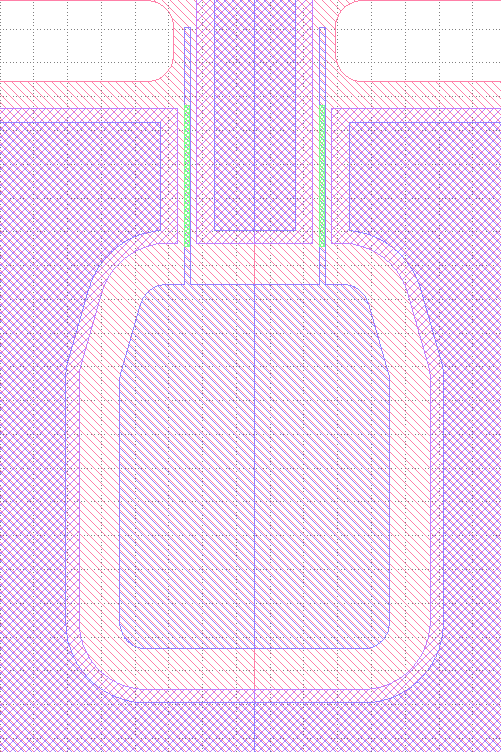
\includegraphics[width=0.36\linewidth]{figures/fabrication_images/enhancement_mode_images/iteration2/old_mask-1.png}
    };

    \node[anchor=north west, inner sep=0pt] (newMask) at ($(oldMask.north east)+(0.08\linewidth,0)$) {
      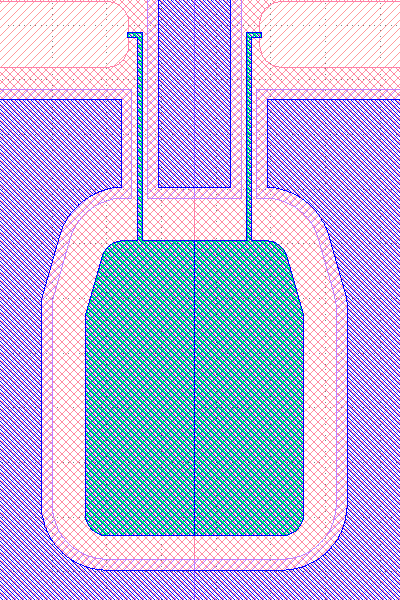
\includegraphics[width=0.36\linewidth]{figures/fabrication_images/enhancement_mode_images/iteration2/new_mask-1.png}
    };

    \node[imglabel, anchor=north, yshift=-1.5mm] at (oldMask.south)
      {Iteration 1 Mask};
    \node[imglabel, anchor=north, yshift=-1.5mm] at (newMask.south)
      {Iteration 2 Mask};

    \draw[change, black!80]
      ($(oldMask.east)+(0.01\linewidth,0)$) --
      ($(newMask.west)+(-0.01\linewidth,0)$);

    \path let \p1=(oldMask.north west), \p2=(oldMask.south east) in
      coordinate (oldBoxNW) at ({\x1+\oldBoxLeft*(\x2-\x1)}, {\y1+\oldBoxTop*(\y2-\y1)})
      coordinate (oldBoxNE) at ({\x1+\oldBoxRight*(\x2-\x1)}, {\y1+\oldBoxTop*(\y2-\y1)})
      coordinate (oldBoxSW) at ({\x1+\oldBoxLeft*(\x2-\x1)}, {\y1+\oldBoxBottom*(\y2-\y1)})
      coordinate (oldBoxSE) at ({\x1+\oldBoxRight*(\x2-\x1)}, {\y1+\oldBoxBottom*(\y2-\y1)});

    \path let \p1=(newMask.north west), \p2=(newMask.south east) in
      coordinate (newBoxNW) at ({\x1+\newBoxLeft*(\x2-\x1)}, {\y1+\newBoxTop*(\y2-\y1)})
      coordinate (newBoxNE) at ({\x1+\newBoxRight*(\x2-\x1)}, {\y1+\newBoxTop*(\y2-\y1)})
      coordinate (newBoxSW) at ({\x1+\newBoxLeft*(\x2-\x1)}, {\y1+\newBoxBottom*(\y2-\y1)})
      coordinate (newBoxSE) at ({\x1+\newBoxRight*(\x2-\x1)}, {\y1+\newBoxBottom*(\y2-\y1)});

    \draw[highlight] (oldBoxNW) rectangle (oldBoxSE);
    \draw[highlight] (newBoxNW) rectangle (newBoxSE);

    \draw[boxarrow]
      ($(oldBoxNE)!0.5!(oldBoxSE)$) --
      ($(newBoxNW)!0.5!(newBoxSW)$);
    \node[connectorlabel] at ($(oldBoxSE)!0.5!(newBoxSW)+(0,-0.20)$)
      {Gate Extended\\to Mesa Edge};
  \end{tikzpicture}

  \vspace{2mm}
  \caption{Mask geometry comparison between Iteration 1 and Iteration 2. The
  Iteration 1 design used two local recess slits between source and drain,
  while the Iteration 2 design expanded the recess across the full gate region
  and adjusted the gate geometry so that it intersected the mesa between source
  and drain.}
  \label{fig:iteration2-mask}
\end{figure}
